\documentclass[11pt,reqno,final]{amsart}

\pdfcompresslevel=0
\pdfobjcompresslevel=0

\usepackage[dvipsnames]{xcolor}% adds colors
\usepackage{amsmath, amsthm}% {amsfonts, amssymb}

% New Characters
\usepackage[latin1]{inputenc}%
\usepackage[T1]{fontenc}

\usepackage{MnSymbol}
\usepackage[normalem]{ulem}% underlining

\usepackage[theoremfont, largesc]{newpxtext} % different text,math font
\usepackage{newpxmath}

\makeatletter
\DeclareMathRadical{\sqrtsign}{symbols}{112}{largesymbols}{112}
\let\sqrt=\undefined
\DeclareRobustCommand\sqrt{\@ifnextchar[\@sqrt{\mathpalette\@x@sqrt}}
\def\@x@sqrt#1#2{%
 \setbox\z@\hbox{$\m@th#1\sqrtsign{\mkern1mu #2}$}
 \mkern3mu\box\z@}
\makeatother




% Page Typesetting
\usepackage[final]{microtype}
\usepackage{relsize}
\usepackage[margin=1in]{geometry}
\usepackage{framed}
\usepackage{tikz}
\usepackage{setspace}
\onehalfspacing

\usepackage{hyperref}
\hypersetup{
  final,
  pdftitle={Math 135 - Written HW 11-06},
  pdfauthor={Bonventre}, 
  linktoc=page,
  pagebackref,
  colorlinks=true,
  citecolor=PineGreen,
  linkcolor=PineGreen,
  linkbordercolor=PineGreen,
}


% Internal References

\usepackage[inline,shortlabels]{enumitem}

% \numberwithin{equation}{section} 
\numberwithin{figure}{section}

\usepackage[nameinlink,capitalise,noabbrev]{cleveref}

\crefname{equation}{}{} % get \cref to behave as \eqref

% \theoremstyle{plain} % bold name, italic text
\newtheorem{theorem}[equation]{Theorem}%
\newtheorem*{theorem*}{Theorem}%
\newtheorem{lemma}[equation]{Lemma}%
\newtheorem{proposition}[equation]{Proposition}%
\newtheorem{corollary}[equation]{Corollary}%
\newtheorem{conjecture}[equation]{Conjecture}%
\newtheorem*{conjecture*}{Conjecture}%
\newtheorem{claim}[equation]{Claim}%
\newtheorem{question}{Question}

\theoremstyle{definition} % bold name, plain text
\newtheorem{definition}[equation]{Definition}%
\newtheorem*{definition*}{Definition}%
\newtheorem{example}[equation]{Example}%
\newtheorem*{example*}{Example}%
\newtheorem{remark}[equation]{Remark}%
\newtheorem{notation}[equation]{Notation}%
\newtheorem{convention}[equation]{Convention}%
\newtheorem{assumption}[equation]{Assumption}%
\newtheorem{exercise}[question]{Exercise}

% ---------- macros
\newcommand{\set}[1]{\left\{#1\right\}}%
\newcommand{\sets}[2]{\left\{ #1 \;|\; #2\right\}}%
\newcommand{\longto}{\longrightarrow}%
\newcommand{\into}{\hookrightarrow}%
\newcommand{\onto}{\twoheadrightarrow}%

\usepackage{harpoon}
\newcommand{\vect}[1]{\text{\overrightharp{\ensuremath{#1}}}}

\newcommand{\del}{\partial}%

\newcommand{\ki}{\chi}
\newcommand{\ksi}{\xi}
\newcommand{\Ksi}{\Xi}

\newcommand{\dlim}{\displaystyle\lim}

% %%%%%%%%%%%%%%%%%%%%%%%%%%%%%%%%%%%%%%%%%%%%%%%%%%%%%%%%%%%%%%%%%%%%%%%%%%%%%%%%%%%%%%%%%%%%%%%%%%%%

\begin{document}

\begin{center}
        \textbf{\Large Math 135, Calculus 1, Fall 2020}\\[10pt]
        {\large Written Homework 11-06}
\end{center}

\thispagestyle{empty}

\renewcommand{\thesection}{\Alph{section}}

\subsection*{Directions:}
Write your solutions neatly and clearly, and submit to Canvas.
In these problems, you should show all of your work in complete mathematical "sentences", writing complete English sentences when you explain your logic.
You are free (and encouraged!) to work with others, but make sure the solutions you write up your solutions indepedently.



\begin{exercise}
        A table of the function values for $f(x)$ and $f'(x)$, and a graph of the piecewise linear function $g(x)$ are shown below.
        \begin{center}
                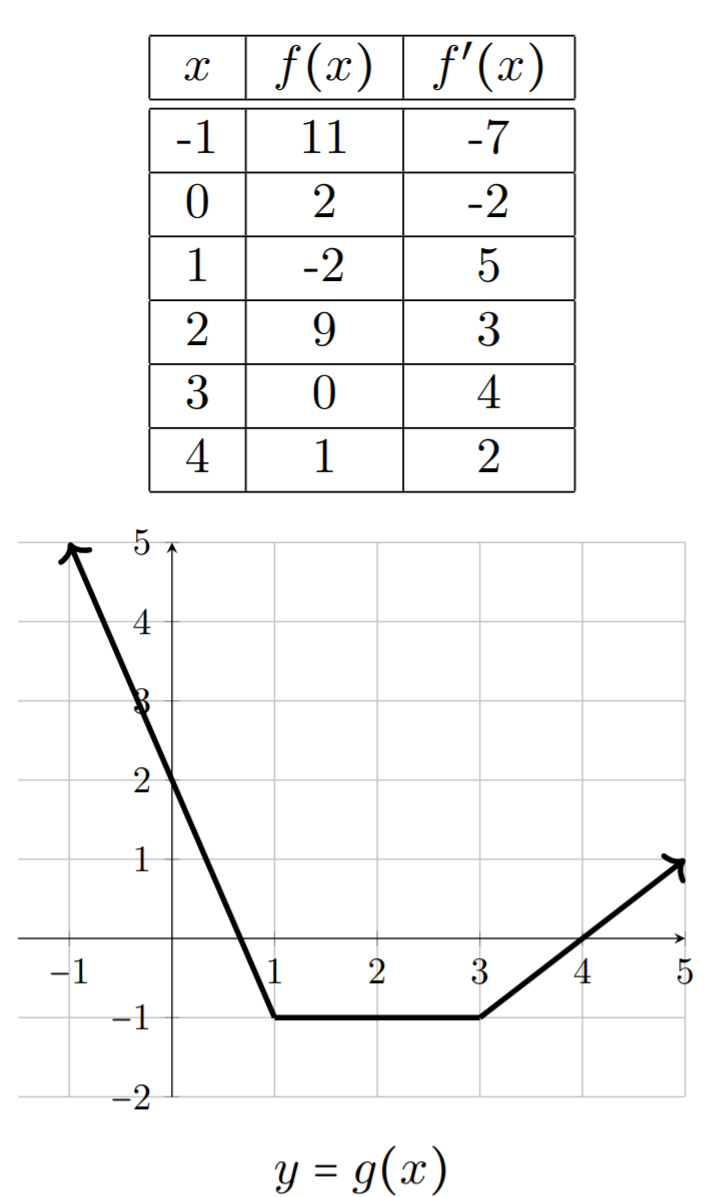
\includegraphics[width=2in]{11-06P_graphs.png}
        \end{center}
        \begin{enumerate}[(a)]
        \item If $h(x) = f(g(x))$, find $h'(0)$.
        \item If $p(x) = (g(x))^3$, find $p'(2)$.
        \item If $k(x) = [g(f(x))]^{2/3}$, find $k'(1)$.
        \end{enumerate}
\end{exercise}

\begin{exercise}
        Find the equations of all tangent lines to the curve $x^2 + 4y^2 = 8$ that pass through the point $(-4,0)$.
\end{exercise}

\begin{exercise}
        Suppose $f$ is a one-to-one differentiable function, and its inverse function $f^{-1}$ is also differentiable.
        Use implicit differentiation to show that
        \[
                \left(f^{-1}\right)'(x) = \dfrac{1}{f'(f^{-1}(x))}.
        \]
\end{exercise}

\end{document}


